%!TEX TS-program = xelatex  
%!TEX encoding = UTF-8 Unicode  
\documentclass[11pt]{article}
\usepackage{xeCJK}
\setmainfont{HiraginoSansGB-W3}
\setCJKmainfont{HiraginoSansGB-W3}
\setCJKsansfont{HiraginoSansGB-W3}

\usepackage{graphicx}
\usepackage{subfigure}
\usepackage{listings}
\lstset{language=C++} 

\begin{document}

\title{Badkid: ELF文件病毒设计报告}
\author{柯嵩宇,陈天垚,万诚,杨闰哲\vspace{1em} \\ 2014级ACM班}
\maketitle

这篇文档的目的,在于还原我们小组对我们的ELF文件病毒“badkid”的设计过程,以及我们在整个设计过程中的技术思考。但请原谅,我们不会在此文中专门介绍ELF文件格式等网上随处可搜到的内容,而是力图忠实地记录我们在实现设计目标中“走过的弯路”与“乍现的灵光”,希望以此给那些想要亲自动手写一个ELF文件病毒(或是想要对抗此类病毒)读者,带来一些有益的启发。

\tableofcontents
\newpage
\section{项目简介}
	~~此项目中,我们的目的是设计一个感染ELF文件的寄生病毒:当一个ELF文件受其感染时,会修改它的头入口点(entry point);当用户运行一个被感染文件时,就会先执行病毒代码,感染同目录下的其他文件,从而达到复制与传播的效果。寄主程序运行顺序的执行顺序如图\ref{fig:order}所示。
	\begin{figure*}[htbp]
		\centering
		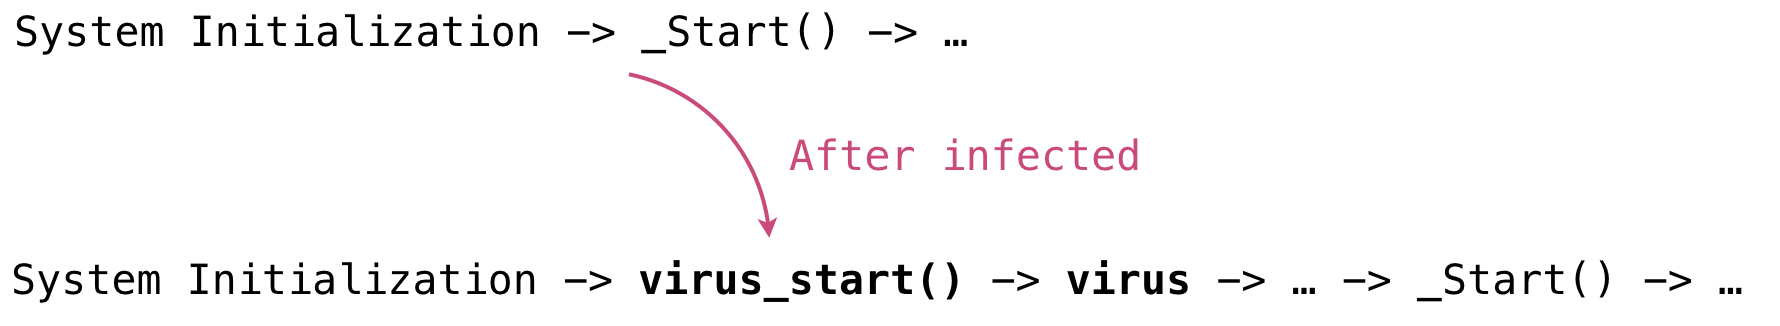
\includegraphics[width = 0.6\textwidth]{figures/fig1_order}
		\caption{受感染寄主程序的执行顺序}
		\label{fig:order}
	\end{figure*}
	
	我们假定病毒工作于以下环境:
	\begin{enumerate}
		\item 指令集架构:x86\_64
		\item 操作系统:Linux
		\item 被感染文件在root权限下运行
	\end{enumerate}
	
	假定一个可获得的root权限,可以让我们专注于ELF文件的分析与重构、病毒的攻击行为与连接病毒本身,而不用操心其他问题。另外,我们选择用C语言写病毒代码,而不是C++,因为C++在编译的时候会包含全局的初始化,这会给改写ELF的过程增添不少麻烦。
	
	
\section{主要技术}
\subsection{初尝试:一个静态病毒?}
\subsection{PIE:位置无关可执行文件}
\subsection{使用一个Wrapper}
\subsection{终极思路:感染共享库}
\section{具体实现}
\subsection{源码解析}
\subsection{一些实验}
\section{小结}

\end{document}
